\documentclass[5pt,landscape]{article}
%\usepackage{fontspec}
%\setsansfont{Roboto Condensed}
\usepackage{multicol}
\usepackage{calc}
\usepackage{ifthen}
\usepackage[landscape]{geometry}
\usepackage{amsmath,amsthm,amsfonts,amssymb}
\usepackage{color,graphicx,overpic}
\usepackage{hyperref}
\usepackage{gensymb}
\usepackage[sfdefault, condensed]{roboto}
\geometry{top=0.3cm,left=0.3cm,right=0.3cm,bottom=0.3cm}


% This sets page margins to .5 inch if using letter paper, and to 1cm
% if using A4 paper. (This probably isn't strictly necessary.)
% If using another size paper, use default 1cm margins.
%\ifthenelse{\lengthtest { \paperwidth = 11in}}
%    { \geometry{top=.5in,left=.5in,right=.5in,bottom=.5in} }
%    {\ifthenelse{ \lengthtest{ \paperwidth = 297mm}}
%        {\geometry{top=1cm,left=1cm,right=1cm,bottom=1cm} }
%        {\geometry{top=1cm,left=1cm,right=1cm,bottom=1cm} }
%    }

% Turn off header and footer
\pagestyle{empty}

% Redefine section commands to use less space
\makeatletter
\renewcommand{\section}{\@startsection{section}{1}{0mm}%
                                {-1ex plus -.5ex minus -.2ex}%
                                {0.5ex plus .2ex}%x
                                {\normalfont\large\bfseries}}
\renewcommand{\subsection}{\@startsection{subsection}{2}{0mm}%
                                {-1explus -.5ex minus -.2ex}%
                                {0.5ex plus .2ex}%
                                {\normalfont\normalsize\bfseries}}
\renewcommand{\subsubsection}{\@startsection{subsubsection}{3}{0mm}%
                                {-1ex plus -.5ex minus -.2ex}%
                                {1ex plus .2ex}%
                                {\normalfont\small\bfseries}}
\makeatother

% Define BibTeX command
\def\BibTeX{{\rm B\kern-.05em{\sc i\kern-.025em b}\kern-.08em
    T\kern-.1667em\lower.7ex\hbox{E}\kern-.125emX}}

% Don't print section numbers
\setcounter{secnumdepth}{0}


\setlength{\parindent}{0pt}
\setlength{\parskip}{0pt plus 0.5ex}

%My Environments
\newtheorem{example}[section]{Example}
% -----------------------------------------------------------------------

\begin{document}
\raggedright
\footnotesize
\begin{multicols*}{5}


% multicol parameters
% These lengths are set only within the two main columns
%\setlength{\columnseprule}{0.25pt}
\setlength{\premulticols}{1pt}
\setlength{\postmulticols}{1pt}
\setlength{\multicolsep}{1pt}
\setlength{\columnsep}{2pt}

\begin{center}
     \Large{\underline{Sensor Principles}} \\
 
\end{center}


% Summary starts here
% --------------------------------------------------------------------------------------
\subsection{A generic sensor interface}
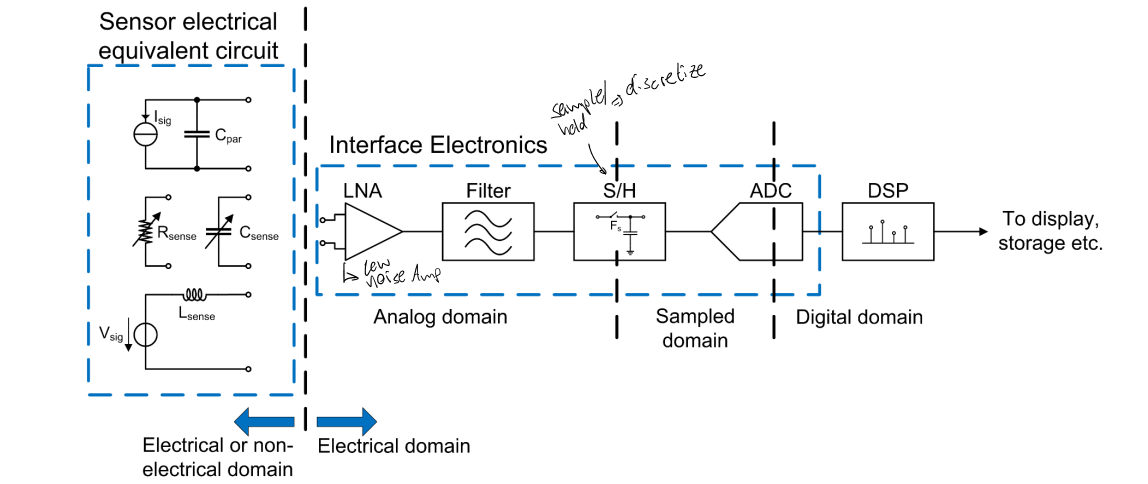
\includegraphics[width = \columnwidth]{images/generic_sensor_interface.png}
\subsection{OPAMP Basics}
\subsection{Opamps in feedback}
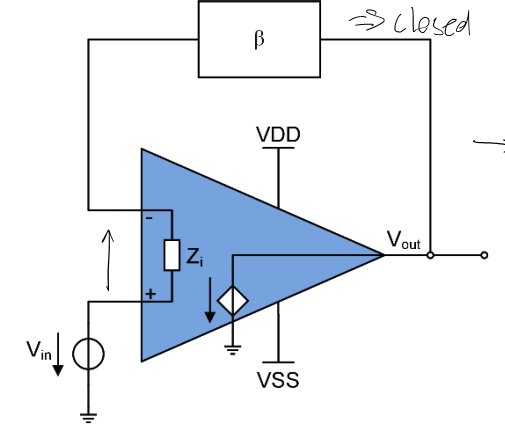
\includegraphics[width = \columnwidth]{images/opampfeedbacl.png}
Gain : $ T(\omega) =\beta \cdot A_0 (\omega $) \\
Phase Margin: $PM =180 \degree + \angle (T(\omega_1)|_{  |T(\omega_1)| = 1 } $
Gain margin:$ GM = 20 \cdot log_{10} (\frac{1}{T(\omega_2)})|_{\angle (T(\omega_2) = - 180 \degree  }$
\textbf{Generic Transfer function}\\
%$ Z_i \rightarrow \infty \Rightarrow V_X = \beta \cdot V_{out} = \beta  $
$  V_{x}=\beta \cdot V_{\text {out }}=\beta \cdot A(\omega) \cdot\left(V_{\text {in }}-V_{x}\right)=\beta \cdot A(\omega) \cdot\left(V_{\text {in }}-\beta \cdot V_{\text {out }}\right)$\\
$ \frac{V_{\text {out }}}{V_{\text {in }}}=\frac{A(\omega)}{1+\beta \cdot A(\omega)} \stackrel{A(\omega)] \gg 1}{\approx} \frac{1}{\beta} $
\textbf{Negative Feedback and linear operation}\\
$ A(\omega) \gg 1 \Rightarrow $ virtual short at the input $ \Delta V \approx 0  $ \\
$ Z_i \rightarrow \infty \Rightarrow i_{oa} \approx 0 $ \\
 Voltage Drive $ \rightarrow $ negative feedback\\
 Current drive $ \rightarrow $ positive feedback 
 \subsection{Errors and Noise}
 \textbf{Limit of detection(LOD):} minimum measurable input amplitude ($ SNR \approx 0 $)  \\
 \textbf{Dynamic range()DR:} ratio of max and min amplitude within inaccuracy levels.\\
 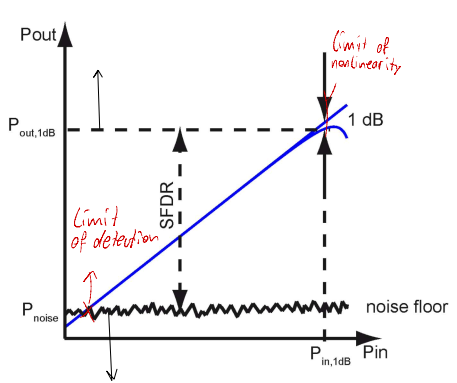
\includegraphics[width = \columnwidth]{images/lod_dr.png}\\
 \textbf{Errortypes}:\\
 Deterministic: source loading, offset, gain error \\
 Random: thermal noise, 1/f noise\\
 \textbf{Quantification}:\\
 Absolute : $ \Delta x=\left|\hat{x}-x_{0}\right| $\\
Relative: $\left|\frac{\Delta x}{x_{0}}\right|=\left|\frac{\hat{x}-x_{0}}{\hat{x}}\right|  $\\
Max inaccuracy: $ \Delta x_{max}| x \in \left[\hat{x}-\Delta x_{\max }, \hat{x}+\Delta x_{\max }\right] $
\textbf{Error Propagation}\\
$ y=f\left(x_{1}, x_{2}, \ldots, x_{N}\right) $\\
Deterministic fluctuations of $ x_i $ $ \rightarrow $ total error:\\
$\Delta y \approx \sum_{i=1}^{N} \frac{\partial f}{\partial x_{i}} \cdot \Delta x_{i}  $\\
Partial derivative $ \frac{\delta f}{\delta x_i} $ is called \textbf{sensitivity}\\
Additive errors are best specified absolute and multiplicative errors are best specified relative \\
\textbf{Interference:}\\
Unwanted coupling of external signal\\
Noise: random fluctuations from setup $ \rightarrow $ can be modeled as error sources
\subsection{Combining Error sources}
\textbf{Output referred noise}\\
Effect of an error-source on the output\\
\textbf{Input referred noise}
Equivalent effect of the error-source on the input\\
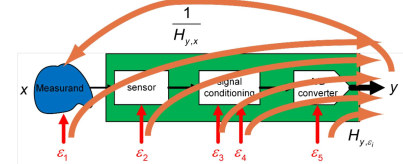
\includegraphics[width = \columnwidth]{images/error_referral.png}\\
Find TF from ES to output $ y:H_{y,ES} \Rightarrow y_{\text {out }, \epsilon_{2}}=H_{y, \epsilon_{2}} \cdot \epsilon_{2}$\\
Refer result back to input wit $ H_{y,x}: x_{\epsilon_{2}}=\frac{y_{\text {out }, \epsilon_{2}}}{H_{y, x}}=H_{y, \epsilon_{2}} \cdot \frac{\epsilon_{2}}{H_{y, x}} $\\
\textbf{Lin. System noise:}\\
$ PSD =  S_{y}(f)=|H(f)|^{2} \cdot S_{x}(f)$
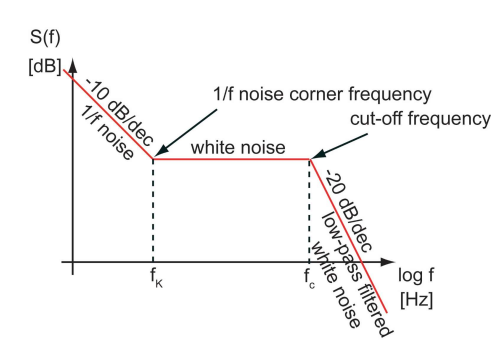
\includegraphics[width = \columnwidth]{images/noise_bode.png}
\subsection{Noise Types}
\textbf{Thermal noise:} excitation of charge carriers(white)\\
\textbf{Shot noise: }carriers randomly crossing the barrier, dependent on DC bias and white \\
\textbf{Flicker Noise:}, due to traps in semiconduct. 1/f spectral density. MOS trans at low freq.\\
\textbf{Thermalnoise Theorem:} Every closed system at temp. T has average. Energy of $ kT/2 $
$ \rightarrow $ $S_{u}(f)=2 k T R($ double-sided $)$ math
$S_{u}(f)=4 k T R($ single-sided $)$ physics
\subsection{Langevin Approach kt/C noise}
PSD noise voltage of $ V_n $ $ = S_{v_{n}}(f)=4 k T \cdot \Re\{Z(j 2 \pi f) $\\
$ \rightarrow $ $ \overline{V_{n}^{2}}=k T\left[\frac{1}{C_{\infty}}-\frac{1}{C_{0}}\right]=\frac{k T}{C} $\\
\textbf{MOS IRN}\\
$ S_{\Delta V_{\text {nG-tot }}^{2}}=4 k T \cdot R_{\text {nG-tot }}, \quad R_{\text {nG-tot }}=\frac{\rho}{W \cdot L \cdot f}+\frac{\gamma_{n D}}{G_{m}} $ with GateExcess Noise factor :$ \gamma_{n D} = (n=1.3) \cdot [0.5 WI; 2/3 SI] $ \\
\textbf{Bipolar Trans IRN:}\\
$ S_{\Delta V_{n R}^{2}}=4 k T \cdot R_{B} $
\subsection{Noise Aanalysis}
small-signal-equivalent is valid.\\
Total ORN: $ S_{n, \text { out }}(f)=\sum_{k=1}^{N}\left|H_{k}(f)\right|^{2} \cdot S_{n k}(f) $\\
N uncorrelated NS.\\
$ H_k(f) $ TF from NS ton output.
IRN: $ S_{V_{\text {neq,IRN }}}(f)=\frac{S_{V_{\text {nout }}}(f)}{|A(f)|^{2}} $ with $ A(f) $ is TF\\
\section{Sensor types}
Information domain $ \rightarrow $ Electrical domain\\
Transduction: Converting a signal from the energy domain into another.\\
Sensors and actuators are transducers\\
\subsection{Sources of eerror}
Noise, sensitivity to unintended quantities, Noise, EMI\\
%\texttt{$ \left(\begin{array}{c}
%E_{\operatorname{mag}} \\
%E_{\text {mech }} \\
%E_{\text {therm }} \\
%E_{\text {opt }} \\
%E_{\text {chem }} \\
%E_{\text {elec }}
%\end{array}\right)= \left(\begin{array}{cccccc}
%\alpha_{\text {mag,mag }} & \alpha_{\text {mag,mech }} & \alpha_{\text {mag,therm }} & \alpha_{\text {mag,opt }} & \alpha_{\text {mag,chem }} & \alpha_{\text {mag,elec }} \\
%\alpha_{\text {mech,mag }} & \alpha_{\text {mech,mech }} & \alpha_{\text {mech,therm }} & \alpha_{\text {mech,opt }} & \alpha_{\text {mech,chem }} & \alpha_{\text {mech,elec }} \\
%\alpha_{\text {therm,mag }} & \alpha_{\text {therm,mech }} & \alpha_{\text {therm,therm }} & \alpha_{\text {therm,opt }} & \alpha_{\text {therm,chem }} & \alpha_{\text {therm,elec }} \\
%\alpha_{\text {opt,mag }} & \alpha_{\text {opt,mech }} & \alpha_{\text {opt,therm }} & \alpha_{\text {opt,opt }} & \alpha_{\text {opt,chem }} & \alpha_{\text {opt,elec }} \\
%\alpha_{\text {chem,mag }} & \alpha_{\text {chem,mech }} & \alpha_{\text {chem,therm }} & \alpha_{\text {chem,opt }} & \alpha_{\text {chem,chem }} & \alpha_{\text {chem,elec }} \\
%\alpha_{\text {elec,mag }} & \alpha_{\text {elec,mech }} & \alpha_{\text {elec,therm }} & \alpha_{\text {elec,opt }} & \alpha_{\text {elec,chem }} & \alpha_{\text {elec,elec }}
%\end{array}\right) \cdot \left(\begin{array}{c}
%E_{\operatorname{mag}} \\
%E_{\text {mech }} \\
%E_{\text {therm }} \\
%E_{\text {opt }} \\
%E_{\text {chem }} \\
%E_{\text {elec }}
%\end{array}\right)+\left(\begin{array}{c}
%E_{\text {mag,os }} \\
%E_{\text {mech,os }} \\
%E_{\text {therm,os }} \\
%E_{\text {opt }, \mathrm{os}} \\
%E_{\text {chem }, \mathrm{os}} \\
%E_{\text {elec }, \mathrm{os}}
%\end{array}\right) $}
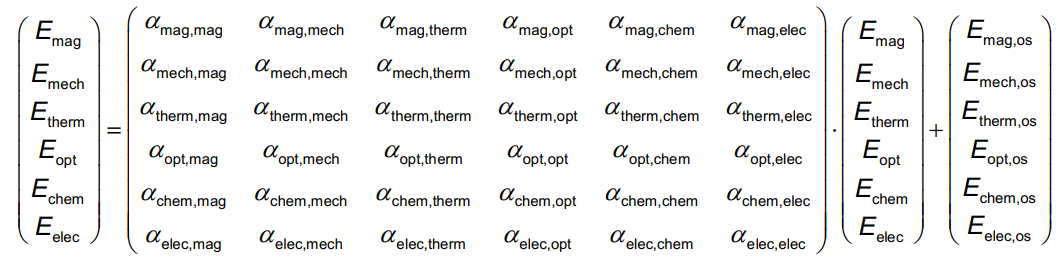
\includegraphics[width = \columnwidth]{images/transconduction_matrix.png}\\
Tandem transducers: Multiple steps to target domain.\\
cross-sensitivity, sensitivity to undesired quantity
\subsection{Sensor classification:}
\textbf{Active Sensors:}\\
Require external source of excitation\\
\textbf{Passive / self-generating sensors:}\\
Generate their own electrical output signal\\
Draws all required energy from the measurand(source loading)
E: Potentiometer for angle measurements.
\textbf{Modulating sensors:}\\
Measure desired quantity by modulating\\
Additional source with modulated energy. Also adds error.
E: Non0contact displacement measrement (rotating disk)\\
\textbf{Analog vs. Digital:}\\
Analog: time and value continuous\\
Digital: Discrete outputs\\
\textbf{Deflection mode sensors:}\\
Response to an output is a deviation from the equilibrium position\\
\textbf{Null mode sensors:}\\
Sensor or instruments exert an influence the measured system opposing the effect of the measurand. Ideally the result is a 0 measurement, typically achieved by feedback. The opposing influence is then the sensor output.
Slower than deflection, but more accurate.\\
\textbf{Resistive sensors - strain gauges}\\
Change in geometry under mechanical stress produces associated resistance change\\
Volum. == const. $ \rightarrow $ $ \frac{\partial V}{V_{0}}=\frac{L_{0}}{V_{0}} \cdot \partial A+\frac{A_{0}}{V_{0}} \cdot \partial L \wedge \frac{\partial V}{V_{0}}=0 \Rightarrow \frac{\partial A}{A_{0}}=-\frac{\partial L}{L_{0}}  $ $ \rightarrow $ $ \frac{\partial R}{R_{0}}=\frac{\partial \rho}{\rho_{0}}+2 \frac{\partial L}{L_{0}} $ $ \rightarrow $$ \frac{\partial R}{R_{0}}=\alpha \cdot \frac{\partial L}{L_{0}}+2 \frac{\partial L}{L_{0}}=\underbrace{(\alpha+2)}_{\triangleq k} \cdot \frac{\partial L}{L_{0}} $\\
k: gauge factor\\
$ \alpha $ proportionality factor $  \frac{\partial \rho}{\rho_{0}} \propto \frac{\partial L}{L_{0}}$
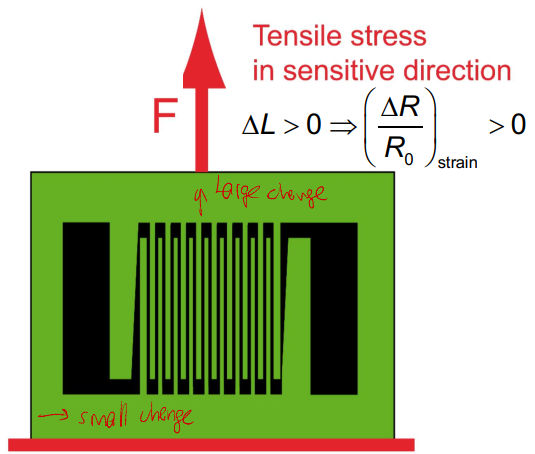
\includegraphics[width = \columnwidth]{images/strain-gauge.png}
\subsection{Readout resistive sensors}
Use a half bridge resistive divider\\
top element sensing resistor
$ \frac{v_{\text {out }}}{V_{\text {bias }}}=\frac{R}{2 R+\Delta R} \Leftrightarrow \frac{\Delta R}{R}=\frac{V_{\text {bias }}}{v_{\text {out }}}-2 $\\
Full bridge to remove offset, 2 sensing elements more sensitive,\\
remove nonlinearity by implementing differential measurements\\
Best use 4point full bridge\\
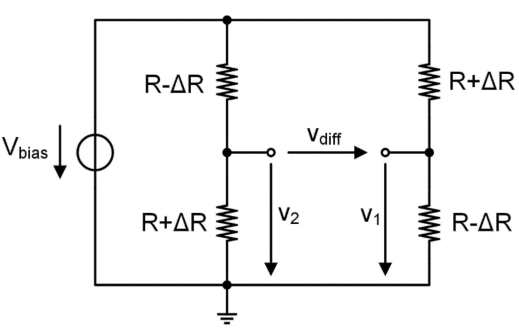
\includegraphics[width = \columnwidth]{images/4point-fullbridge.png}\\
$ V_{\mathrm{diff}}=v_{2}-v_{1}=\frac{\Delta R}{R} \cdot V_{\mathrm{bias}} $\\
Sensitivity $ S = 45mV/V$ excitation for 1V input\\
Accuracy $ A = \frac{v_{\mathrm{diff}}\left(\frac{\Delta R}{R}\right)-V_{\mathrm{diff}, \text { lin }}\left(\frac{\Delta R}{R}\right)}{V_{\mathrm{diff}}\left(\frac{\Delta R}{R}\right)} $ \\
Deviation from the ideal bridge
\subsection{BridgeParameters}
\textbf{Bridge resistance: } Unloaded $ R $ across the signal terminals\\
\textbf{Offset error} Outputvoltage at 0 input\\
\textbf{Drift:} Outputchange conditioned on environmental condition
\subsection{Differential/ Commonmode signals}
\textbf{Recall:} $ V_{1}=\frac{1}{2} \cdot\left(1-\frac{\Delta R}{R}\right) \cdot V_{\text {bias }}, \quad v_{2}=\frac{1}{2} \cdot\left(1+\frac{\Delta R}{R}\right) \cdot V_{\text {bias }} $\\
\textbf{Differential signal:} $ V_{\mathrm{diff}}=V_{2}-V_{1}=\frac{\Delta R}{R} \cdot V_{\mathrm{bias}} $\\
\textbf{Common-mode signal:} $ V_{\mathrm{CM}}=\frac{v_{2}+v_{1}}{2}=\frac{V_{\text {bias }}}{2} $
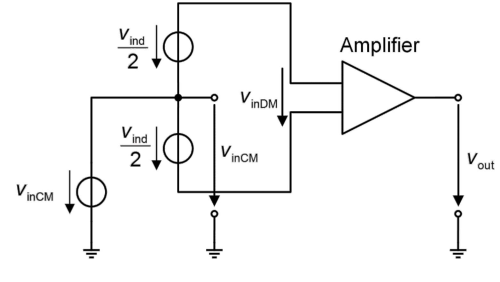
\includegraphics[width=\columnwidth]{images/common_mode_amp.png}\\
\textbf{DiffGain:} $ V_{\text {out }}=A_{\text {DM }} \cdot V_{\text {inDM }} $\\
\textbf{CMMGain:} $ V_{\text {out }}=A_{\mathrm{CM}} \cdot v_{\text {inCM }} $\\
Ideally $ A_{cm} $ is 0 or $ A_{cm} \ll  A_{dm}$\\
Commonmode rejection ratio(CMRR): $ \mathrm{CMRR} \triangleq\left|\frac{A_{\mathrm{DM}}}{A_{\mathrm{CM}}}\right|=\left|\frac{\mathrm{d} v_{\mathrm{out}} / \mathrm{d} v_{\mathrm{inDM}}}{\mathrm{d} v_{\mathrm{out}} / \mathrm{d} v_{\mathrm{inCM}}}\right| $\\
Often in \textbf{dB}\\
\textbf{Opampbase difference aplifier:}\\
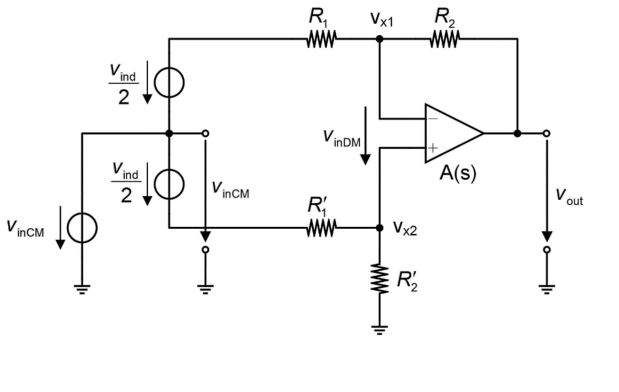
\includegraphics[width=\columnwidth]{images/diffbased_opamp.png}\\
1st: $ A(s) = \infty, R_2 = R_2' = \alpha \cdot R_1 = \alpha R_1'$\\
$ A_{DM} = - \alpha, A_{CM} =0, CMRR = \infty $ \\
$ \begin{array}{l}
2^{\text {nd }} \text { assume } A(s)=\infty, R_{2}=\alpha \cdot R_{1}, \\
R_{2}^{\prime}=(\alpha+\Delta \alpha) \cdot R_{1}^{\prime}, R_{1}^{\prime}=R_{1}+\Delta R
\end{array} $
$ 
A_{\mathrm{DM}} =-\left( \alpha+\frac{\Delta \alpha}{2 \cdot(1+\alpha+\Delta \alpha)} \right)$ \\
$A_{\mathrm{CM}} =\frac{\Delta \alpha}{1+\alpha+\Delta \alpha} $\\
$\mathrm{CMRR} =-\frac{1}{2}+\frac{\alpha \cdot(1+\alpha+\Delta \alpha)}{\Delta \alpha}
$\\
3d: $ A(s)=A_{\mathrm{DC}} /\left(1+s \cdot \frac{A_{\mathrm{DC}}}{\mathrm{GBW}}\right) $\\
$ A_{\mathrm{DM}} =-\left(\alpha+\frac{\Delta \alpha}{2 \cdot(1+\alpha+\Delta \alpha)}\right) \cdot \frac{1}{1+\frac{1}{A_{\mathrm{DC}}}+\frac{\alpha}{A_{\mathrm{DC}}}+(1+\alpha) \cdot \frac{s}{\mathrm{GBW}}} $\\
$A_{\mathrm{CM}} =\frac{\Delta \alpha}{1+\alpha+\Delta \alpha} \cdot \frac{1}{1+\frac{1}{A_{\mathrm{DC}}}+\frac{\alpha}{A_{\mathrm{DC}}}+(1+\alpha) \cdot \frac{s}{\mathrm{GBW}}}$ \\
$\mathrm{CMRR} =-\frac{1}{2}+\frac{\alpha \cdot(1+\alpha+\Delta \alpha)}{\Delta \alpha}$
\section{Magnetic Field Sensors}
$ V_{\text {hall }}=G \cdot \frac{\mu \cdot \rho}{h} \cdot l \cdot B=G \cdot \frac{1}{e \cdot n \cdot h} \cdot l \cdot B=S_{l} \cdot l \cdot B $
G: geometry factor
\textbf{Noise sources:}\\
- Thermal noise\\
-1/f noise \\
-Noise of conditioning electronics\\
Noise power: $ V_{noise} \sqrt{4kT \cdot R \cdot \Delta f} $\\
Signal power: $ V_{hall} S_I \cdot I \cdot B $\\
Resolution: $ B_{\min } \hat{\wedge} \frac{V_{\text {noise }}}{V_{\text {hall }} / B}=\frac{\sqrt{4 k T \cdot R \cdot \Delta f}}{S_{l} \cdot I} $\\
With $ S_I = \frac{\mu \cdot \rho}{h\cdot e \cdot n} \cdot G $\\
At $ B=0 $ Hall plate can be modeled as wheatstone bridge, non-uniform stress causes intrinsic offset(5 to 30mT)\\
Cancel intrinsic offset by coupling $ \degree  $ turned sensors, current and sense ports are swapped\\
Idea: Hall voltage is in phase and gradient caused offsets are than $ 180 \degree $ out of phase\\
\textbf{Spinning current method:}\\
Sense and current ports are switched every clock cycle\\
Idea: A DC component equal to the offset and a frequency component proportional to the hall voltage is produced \textbf{(Fourier Expansion of a square wave})\\
By modulating the information to the clock frequency noise and offset are greatly mitigated.\\
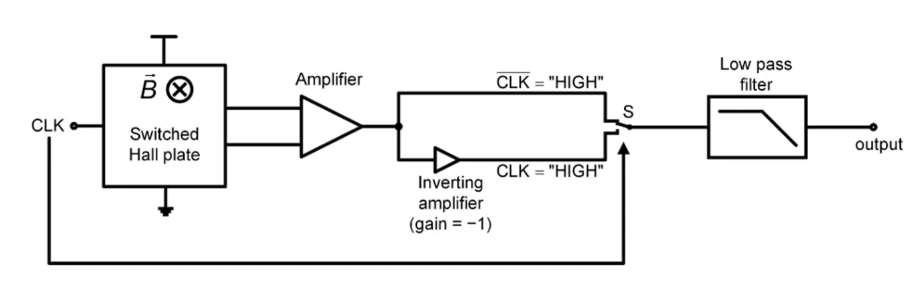
\includegraphics[width=\columnwidth]{images/switched_hall_system.png}
Multiplying by 1 and -1 to demodulate back to low frequency. \\
Low pass stage to remove signal around the 2nd harmonic\\
This allow to see the base noise floor of the sensor not 1/f noise.\\
In the conventional implementation 2 bias currents are used in the low power configuration the bias form the plate is reused for the amplifier.\\
\subsection{Temperature Sensors}
Seebeck effect: Convert temp. gradient to electromotive force
$ F(T)  \hat{=} \int_{T_{stand.}}^{T} (S_{+} (T') - S_- (T')) dT'   $ $ \rightarrow $ $ E_{emf} = F(T_{sense} - F(T_{ref})$
\textbf{Temperature stable references:}\\
$ V_{\mathrm{REF}}(T)=V_{\mathrm{CTAT}}(T)+K \cdot V_{\mathrm{PTAT}}(T) $\\
Bandgap reference:
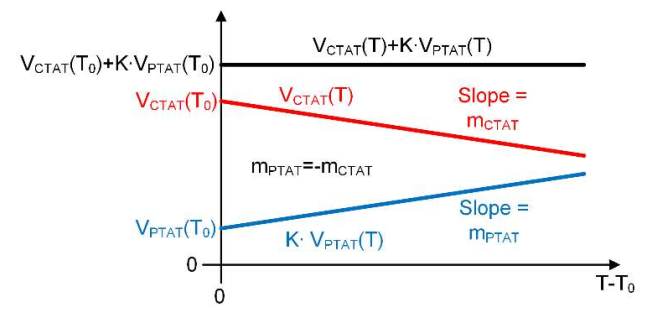
\includegraphics[width=\columnwidth]{images/bandgapreference.png}
PTAT: Proportional to absolute temperature\\
CTAT: Complementary to absolute temperature\\
Scale one slope and add the function for a temp. constant reference\\
This can be built with a diode or a BJT with a shorted base and collector\\
Butt current is also temperature dependent so use diff pair.
$ V_{\text {PTAT }}=\Delta V_{\text {EB }}=V_{\text {EB1 }}-V_{\text {EB2 }} \approx $\\
$ \frac{k T}{q} \cdot \ln \left[\frac{I_{q} \cdot I_{S}^{\prime} \cdot A_{E 2}}{I_{S}^{\prime} \cdot A_{E 1} \cdot I_{q}}\right]=\frac{k T}{q} \cdot \ln \left[\frac{A_{E 2}}{A_{E 1}}\right] $\\
Scale currents or diodes to make equal bias\\
$ V_{\mathrm{EB}}=\underbrace{E_{g} / q}_{V_{G}}-\underbrace{\frac{k T}{q}}_{U_{T}} \cdot \ln \left(\frac{I_{s}^{\prime}}{I_{D}}\right)=V_{G}-U_{T} \cdot \ln \left(\frac{K_{1} \cdot T^{\gamma}}{I_{D}}\right) $\\
$ V_G \approx V_{G0K} - a \cdot T  $\\
With $ I_S' > I_D $ but also temperature dependent $ \rightarrow $ curved CTAT.\\
\textbf{Combine CTAT and PTAT:}
Series: $ V_{\mathrm{REF}}=I_{\mathrm{PTAT}} \cdot R_{2}+V_{\mathrm{CTAT}}=\frac{R_{2}}{R_{1}} \cdot V_{\mathrm{PTAT}}+V_{\mathrm{CTAT}} $\\
Parallel: $ V_{\mathrm{REF}}=\left(I_{\mathrm{PTAT}}+I_{\mathrm{CTAT}}\right) \cdot R_{3}=\frac{R_{3}}{R_{1}} \cdot V_{\mathrm{PTAT}}+\frac{R_{3}}{R_{2}} \cdot V_{\mathrm{CTAT}} $\\
\subsection{Capa. Sensor Readout}
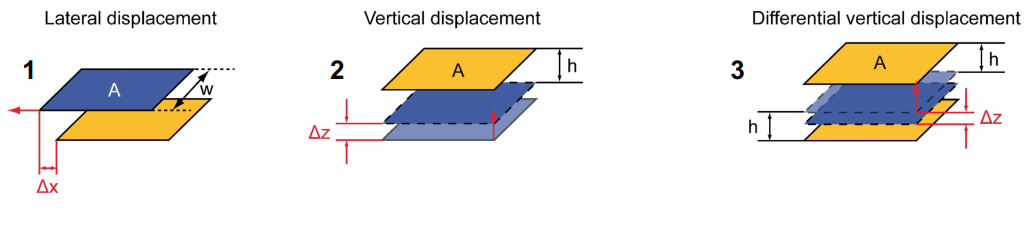
\includegraphics[width=\columnwidth]{images/capa_sensors.png}
1: $ \Delta C=C-C_{0}=\varepsilon \cdot \frac{W}{h} \cdot \Delta x $\\
2: $ \Delta C =  \frac{\varepsilon \cdot A}{h} \cdot \frac{\Delta z / h}{1+\Delta z h} \approx \frac{\varepsilon \cdot A}{h^{2}} \cdot \Delta z$\\
3: $ \Delta C = \varepsilon \cdot \frac{A}{h} \cdot\left(\frac{2 \cdot \Delta z / h}{1-[\Delta z / h]^{2}}\right)=\frac{2 \cdot \varepsilon \cdot A}{h^{2}} \cdot \Delta z $\\
\textbf{OpenLoop readout:} \\
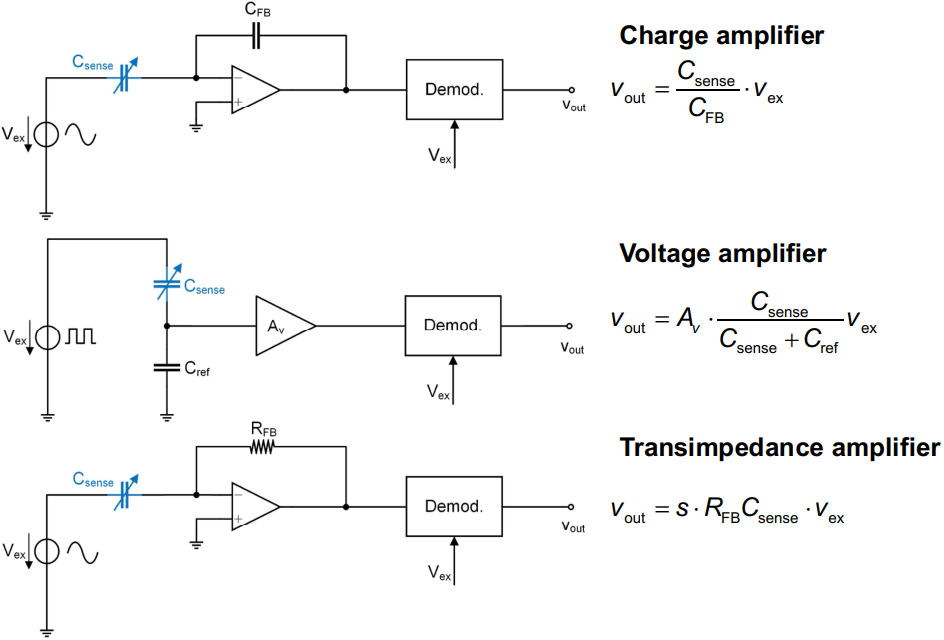
\includegraphics[width=\columnwidth]{images/amplifier_capa.png}
\textbf{ChargeAmp:}$ V_{\text {out }}=\frac{C_{\text {sense }}}{C_{\mathrm{FB}}} \cdot V_{\mathrm{ex}} $
\textbf{ChargeAmpNonideal:}$ \frac{V_{\text {out }}}{V_{\text {in }}}=-\frac{j \omega \cdot R_{\mathrm{FB}} C_{\text {in }}}{\left(1+\frac{j \omega}{\mathrm{GBW}}\right) \cdot\left(1+\frac{j \omega}{\omega_{\mathrm{FB}}}\right)} $\\
\textbf{VoltAmp:} $ v_{\text {out }}=A_{v} \cdot \frac{C_{\text {sense }}}{C_{\text {sense }}+C_{\text {ref }}} V_{\text {ex }} $\\
\textbf{TransImpAmp:} $ v_{\text {out }}=s \cdot R_{\mathrm{FB}} C_{\text {sense }} \cdot v_{e x} $\\
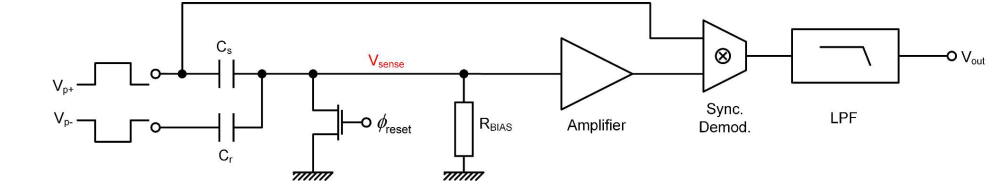
\includegraphics[width=\columnwidth]{images/dc_pot_capa.png}\\
$ V_{Sense} $ not grounded sensitive to leakage currents\\
Bias resistor provides well defined DC-point. $ R_{Bias} $ needs to be large because of the highpass forming, corner frequency needs to be low enough compared to excitation freq. \\
Periodic reset can also be used where $ V_{p+} = V_{p-} =0  $\\
Correlated double sampling can also bes used:\\
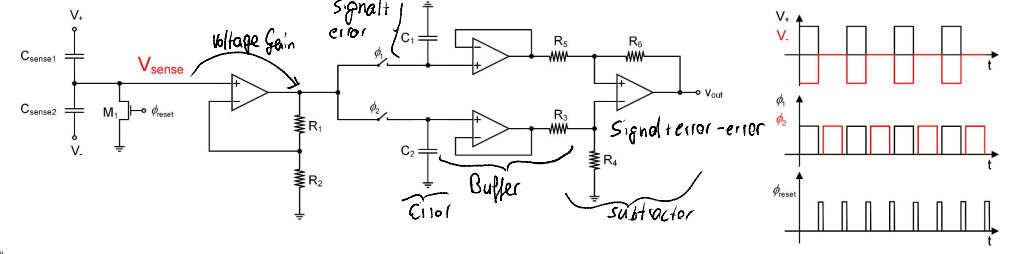
\includegraphics[width=\columnwidth]{images/corr_double_sample.png}\\
\textbf{Bootstrapping: VoltAmp}\\
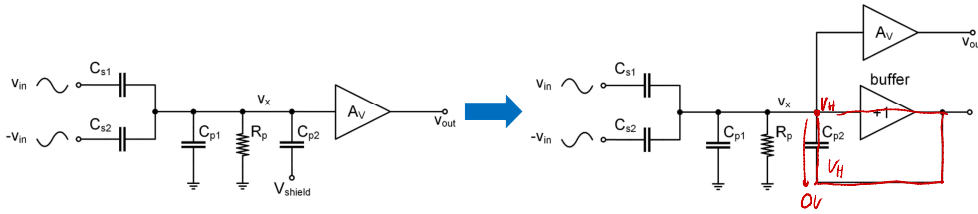
\includegraphics[width=\columnwidth]{images/bootstrapping.png}\\
$ C_{s 1}=C_{s 0}+\Delta C / 2 $$ C_{s 2}=C_{s 0}-\Delta C / 2 $, $ v_{out} $ becomes sensitive to parasitic capacitance\\
Can be bootstrapped out with voltage buffer driving $ V_{shield} $\\
$ v_{\text {out }}=\frac{\Delta C}{2 C_{\mathrm{s} 0}+C_{\mathrm{p} 1} +(C_{p2})} \cdot A_{v} \cdot v_{\text {in }} $ $ C_{p2} $ gets removed by $V_{shied} $\\
Can also use TIA, the virtual ground helps with the parasitic capacitance, this also works in the charge amplifier\\
\textbf{DiffReadoutChargeAmp:}j
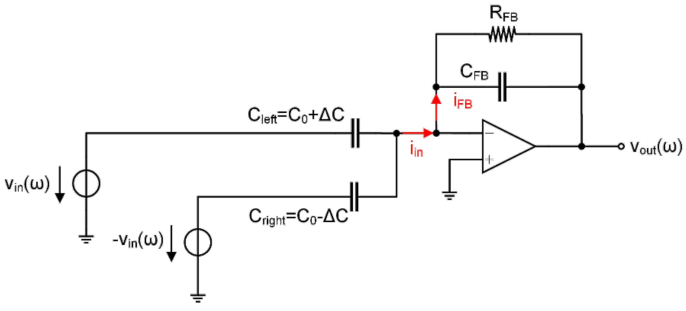
\includegraphics[width=\columnwidth]{images/diff_readout_chargeamp.png}\\
\textbf{Req $ V_{ex} $:}\\
Error will propagate to output directly\\
Accuracy more important for small $ \Delta C $\\
Mismatch or drift will introduce errors\\
Sinewave can be created with center-tapped transformer or active balun\\
Rectangular witch switched excitation schemes\\
\textbf{DiffReadoutChargeAmp:}
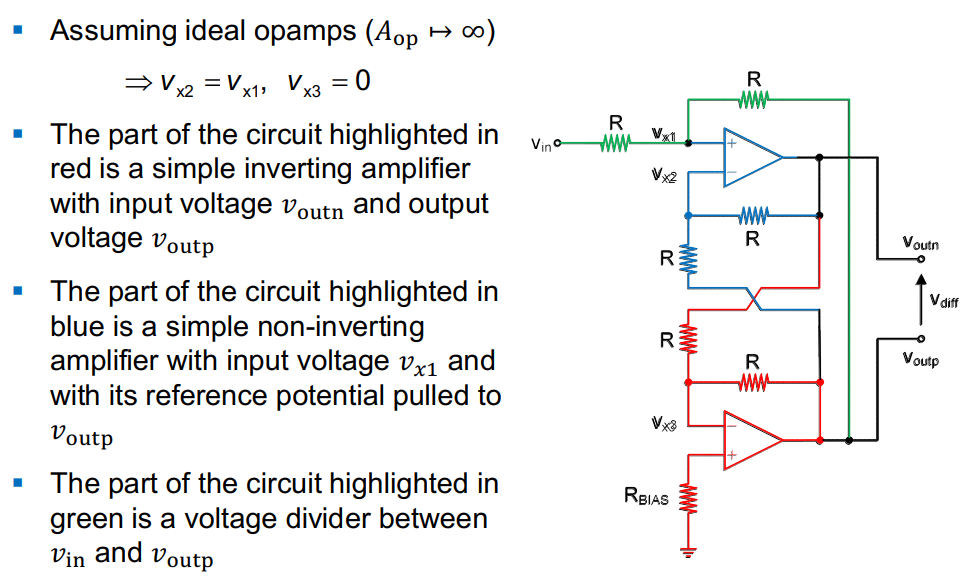
\includegraphics[width=\columnwidth]{images/active_balun.png}\\
$ V_{\text {outp }}=V_{\text {in }}=-V_{\text {outn }} $\\
\textbf{Differential Capa sensing:}\\
$ \Delta v_{x, \text { amp }} \approx-\frac{\Delta x}{x_{0}} \cdot V_{\mathrm{ex}} $\\
\textbf{Resonant readout:}\\
$ \omega_{\mathrm{LC}}=\frac{1}{\sqrt{L_{\text {coil }} \cdot C_{s}}} $\\
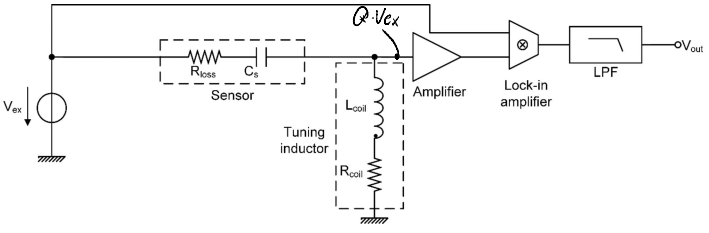
\includegraphics[width=\columnwidth]{images/reso_readout_capa.png}\\
\textbf{DoubleDiffReadout:}
$ \Delta V_{\text {out }}=-\Delta V_{e x} \cdot(\frac{\Delta C_{s}}{C_{i}} \cdot \underbrace{\left[1-\frac{C_{s}}{C_{s}+C_{i}+C_{p}}\right]}_{\text {gain error }}-\underbrace{\frac{\Delta C_{i}+\Delta C_{p}}{C_{i}} \cdot \frac{C_{s}}{C_{s}+C_{i}+C_{p}}}_{\text {offset error }}) $
\section{Differential Measurements}
- Inherent rejection to common-mode interference ans noise\\
- Wider Signal swing for a given supply voltage\\
- Minimum effect of even order distortion including DC offset\\
- Can lead to improved sensor linearity \\
But respond to some degree to common mode signal\\
\textbf{Ideal DiffPair:}\\
CMMR: $  \triangleq 20 \cdot \log \left(\left|\frac{A_{\mathrm{DM}}}{A_{\mathrm{CM}-\mathrm{to}-\mathrm{DM}}}\right|\right) =20 \cdot \log \left(\frac{2 G_{\operatorname{mav}} \cdot r_{\mathrm{out}}}{\Delta R_{L} / R_{\mathrm{Lav}}+\Delta G_{\mathrm{m}} / G_{\mathrm{mav}}}\right] $\\
PSRR: $ \triangleq 20 \cdot \log \left(\left|\frac{A_{\mathrm{DM}}}{A_{\mathrm{vDD}}}\right|\right)=20 \cdot \log \left(\left|\frac{A_{\mathrm{DM}}}{\Delta V_{\mathrm{out}} / \Delta \mathrm{VDD}}\right|\right) $
Process variation causes mismatch between resistors and current source is not ideal\\
Input referred offset is the voltage needed to get zero volts differential output\\
IRO: $ \Delta V_{G}=V_{\mathrm{OS}}=-\frac{I_{\mathrm{Dav}}}{G_{\mathrm{mav}}} \cdot\left(\frac{\Delta R_{\mathrm{L}}}{R_{\mathrm{Lav}}}+\frac{\Delta \beta}{\beta_{\mathrm{av}}}\right)-\Delta V_{\mathrm{TO}} $
OffsetVoltage: 10mV \textbf{MOS} ; 1mV \textbf{BJT}, 120 $ \mu  $, trimmed BJT
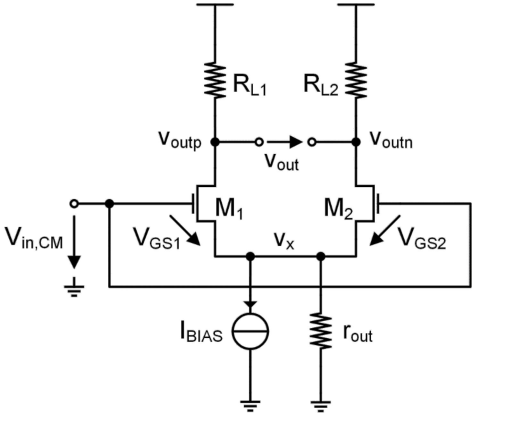
\includegraphics[width=\columnwidth]{images/cmrr_diff_pair.png}\\
$ CMRR \cdot V_{os} \approx G_{mav} \cdot r_{out} \cdot V_{OV} $, $ V_{OV} = \frac{I_{DAV}}{G_{mav}} $
\textbf{PSRR:}\\
$ \mathrm{PSRR}_{\mathrm{vDD}} \cong G_{\operatorname{mav}} R_{\mathrm{Lav}} /\left(g_{\mathrm{outM} 1,2} \cdot\left(\frac{g_{\mathrm{out}}}{G_{\mathrm{mav}}} \cdot \Delta R_{\mathrm{L}}-2 \cdot R_{\mathrm{Lav}} \cdot \frac{\Delta G_{\mathrm{m}}}{G_{\mathrm{mav}}}\right)\right. $\\
$ \mathrm{PSRR}_{\mathrm{vss}} \cong G_{\operatorname{mav}} \cdot R_{\mathrm{Lav}} / g_{\mathrm{out}} \cdot\left(\Delta R_{\mathrm{L}}+R_{\mathrm{Lav}} \cdot \frac{\Delta G_{\mathrm{m}}}{G_{\mathrm{mav}}}\right) $
\section{Modulation}
Stnontms: Coherent detectrion, synchronous demodulation, lock-in amplification, chopping\\
All modulation techniques, square wave is called chopping\\
Leads to better low freq. specification, smaller 1/f, bigger CMRR and PSRR\\
\textbf{Trimming:} Measuring static error offset and gain and adjusting the value of a component to reduce the error to 0\\
Low complexity, no bandwith limit, but reqs. measure equipment\\
Also reqs. memory element\\
\textbf{Dyn. offset cancel:}\\
usually no measure eq. but more complex circuits, reduce bandwidth\\
\textbf{AutoZeroing:}\\
periodically measure offset and substract from input(time domain)\\
\textbf{Chopping:}\\
Modulate signal above 1/f noise(freq. domain)\\
\textbf{Chopper Amps}\\
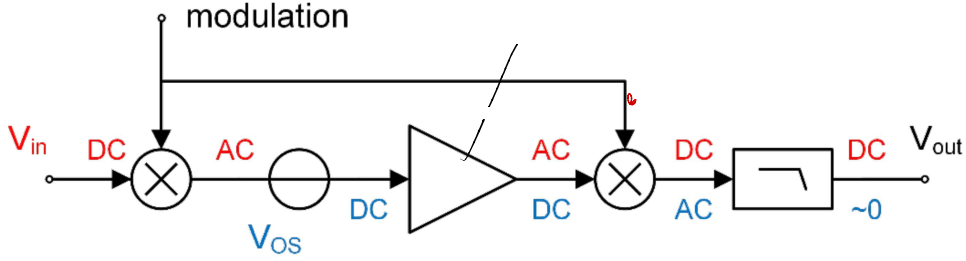
\includegraphics[width=\columnwidth]{images/chop_amp.png}\\
implemented with polarity reversing switch\\
\textbf{Time-Domain-Chopping:}\\
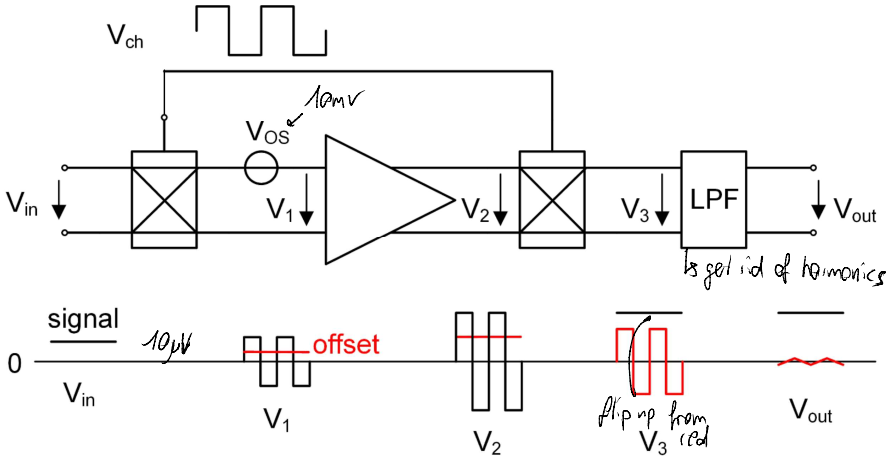
\includegraphics[width=\columnwidth]{images/time_domain_chopping.png}\\
Complete suppression of 1/f noise if $ f_{chop} > 1/f $ corner freq., but up-modulated offset must be filtered out. loss of bandwidth and residual chopper ripple.
\textbf{Charge Injection}\\
Injected charge splits half-half\\
Charge: $ Q=W \cdot L \cdot C_{\mathrm{ox}} \cdot\left[V_{\varphi}-V_{\mathrm{in}}-V_{\mathrm{T} 0}\left(\sqrt{V_{\mathrm{in}}}\right)\right] $\\
Linear w.r.t to $ W\cdot L $ non-linear w.r.t. $ V_{in} $
$ V_{\text {out }}=V_{\text {in }}(1+\underbrace{\frac{W \cdot L \cdot C_{o x}}{2 C_{L}}}_{\text {gain error }})-\underbrace{\frac{W \cdot L \cdot C_{o x}}{2 C_{L}} \cdot\left[V_{\varphi}-V_{T 0}\left(\sqrt{V_{\text {in }}}\right)\right]}_{\text {offset \& dostortion }} $\\
\textbf{Clock feedthrough}\\
Overlap capacitance of trans.: $ C_{OV} $\\
$ \Delta V_{\text {out }}=\frac{C_{\text {ov }}}{C_{\text {ov }}+C_{L}} \cdot V_{\varphi} $\\
Asymmetric clock duty cycle causes demodulation signal to have DC component which feeds through\\
\textbf{Bandwidth gain acc}\\
Limited applifier Bandwidth causes output signal to not be perfectly square, therefore less gain\\
\textbf{AutoZeroing}\\





\end{multicols*}
\end{document}






























